\documentclass[preview]{standalone}
\usepackage{tikz,fullpage,tikz-network,verbatim}
\usetikzlibrary{arrows, petri, topaths, calc, angles, quotes}
\begin{document}
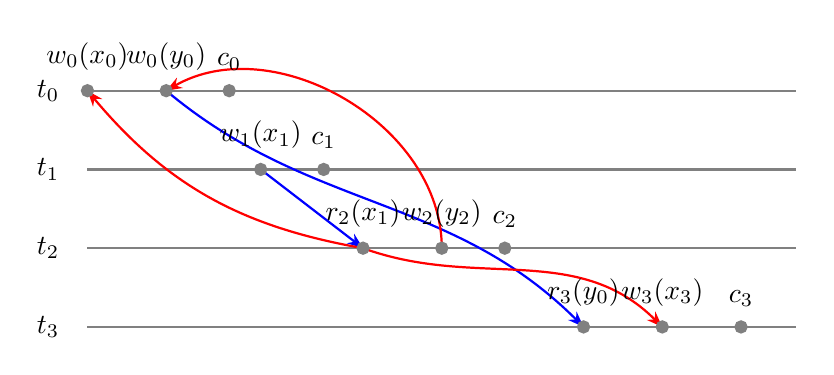
\begin{tikzpicture}[scale=1,transform shape,
>={Stealth[round]},thick,black!50,text=black,
every new ->/.style={shorten >=1pt},
graphs/every graph/.style={edges=rounded corners}]

  % \draw (0, 0) grid (10, 5);
  
  \draw (0.5, 4) node {$t_0$} (1, 4) -- (10, 4) node { };
  \draw (0.5, 3) node {$t_1$} (1, 3) -- (10, 3) node { };
  \draw (0.5, 2) node {$t_2$} (1, 2) -- (10, 2) node { };
  \draw (0.5, 1) node {$t_3$} (1, 1) -- (10, 1) node { };
 
  % m = w_0(x_0) w_0(y_0) c_0 w_1(x_1) c_1 r_2(x_1) w_2(y_2) c_2 r_3(y_0) w_3(x_3) c_3
  \coordinate (w0x0) at (1  ,4);
  \coordinate (w0y0) at (2  ,4);
  \coordinate (c0)   at (2.8,4);
  \coordinate (w1x1) at (3.2,3);
  \coordinate (c1)   at (4  ,3);
  \coordinate (r2x1) at (4.5,2);
  \coordinate (w2y2) at (5.5,2);
  \coordinate (c2)   at (6.3,2);
  \coordinate (r3y0) at (7.3,1);
  \coordinate (w3x3) at (8.3,1);
  \coordinate (c3)   at (9.3,1);

  % mvcs = {(r_2(x_1), w_3(x_3))}
  \draw [blue,->,-{Stealth[length=2mm]}] (w0y0) to [out=320] (r3y0);
  \draw [blue,->,-{Stealth[length=2mm]}] (w1x1) -- (r2x1);
  \draw [red,->,-{Stealth[length=2mm]}] (r2x1) to [out=170,in=310] (w0x0);
  \draw [red,->,-{Stealth[length=2mm]}] (r2x1) to [out=340] (w3x3);
  \draw [red,->,-{Stealth[length=2mm]}] (w2y2) to [out=90,in=30] (w0y0);

  % step graph
  \filldraw (w0x0) circle [radius=2pt] node [label=above:$w_0(x_0)$] {};
  \filldraw (w0y0) circle [radius=2pt] node [label=above:$w_0(y_0)$] {};
  \filldraw (c0)   circle [radius=2pt] node [label=above:$c_0$] {};
  \filldraw (w1x1) circle [radius=2pt] node [label=above:$w_1(x_1)$] {};
  \filldraw (c1)   circle [radius=2pt] node [label=above:$c_1$] {};
  \filldraw (r2x1) circle [radius=2pt] node [label=above:$r_2(x_1)$] {};
  \filldraw (w2y2) circle [radius=2pt] node [label=above:$w_2(y_2)$] {};
  \filldraw (c2)   circle [radius=2pt] node [label=above:$c_2$] {};
  \filldraw (r3y0) circle [radius=2pt] node [label=above:$r_3(y_0)$] {};
  \filldraw (w3x3) circle [radius=2pt] node [label=above:$w_3(x_3)$] {};
  \filldraw (c3)   circle [radius=2pt] node [label=above:$c_3$] {};
\end{tikzpicture}
\end{document}
